\documentclass[12]{article}
\usepackage[utf8]{inputenc}
\usepackage{cite}
\usepackage{float}
\usepackage{graphicx}
\usepackage{amssymb}
\author{Xavier Martín Ballesteros and Adrià Cabeza Sant'Anna \\ \small UNIVERSITAT POLITÈCNICA DE CATALUNYA}
\title{Meat Quality Control \\ \large{Computer Vision, UPC}}


\begin{document}

%\maketitle

\begin{titlepage}
	\centering
%	{\scshape\LARGE UNIVERSITAT POLITÈCNICA DE CATALUNYA \par}
	\vspace{1cm}
	{\scshape\Large UNIVERSITAT POLITÈCNICA DE CATALUNYA\par}
	\vspace{1.5cm}
	{\huge\bfseries Computer Vision \par}
	\vspace{2cm}
	{\Large \textbf{Meat Quality Control}\par}
	\vspace{0.2cm}
	{\Large Adrià Cabeza Sant'Anna and Xavier Martin Ballesteros\break \par}
	
	\vspace*{\fill}
	
\includegraphics[scale=0.4]{UPClogo.png}\par\vspace{1cm}

% Bottom of the page
	{\large \today}
\end{titlepage}

\newpage
\tableofcontents
%podem posar un \newpage aquí si volem 

\section{Introduction}
The aim of this assignment is to detect the percentage of fat in the images with chops using binarization.

We have first computed a mask that only selects the chop pixels. To do it, we have used Otsu thresholding method. Once we have got the part of the image we wanted, we have used several  techniques to calculate the threshold. Binarize the image with this threshold leaves in blank the fat pixels, which is what we wanted. Then, dividing the pixels of fat by the chop pixels, we got the percentage of fat in a specific chop. Moreover, we have also computed manually both thresholds (chop and fat) using the histogram obtained.

The methods consists in setting a constant value called \textit{threshold} ($T$) and split up the pixels depending on its value ($ f(i,j)$):
\vspace{-0.6cm}
\begin{center}
$$ g(i,j)=1\ if\ f(i,j) \geq T$$ 
$$ g(i,j)=0\ if\ f(i,j) \leq T$$
\end{center}

In the following sections we will introduce different methods to find the threshold value and compare its results.

\section{Binarization}
\subsection{Basic Binarization}
This is the first method we tried and also the fastest and easiest one. 

\noindent Our approach was to print the histogram of the picture and check where we could set the best value for the \textit{threshold} in order to split up the fat. The histograms that we got were bimodal so we could set an acceptable value just by looking at it. We believe that this distribution of pixel values is formed because we are working with grayscale pictures of chops where we can appreciate clearly a lighter tone for the fat and darker tones for the rest.
\subsection{P-tile Method}
This method uses knowledge about the area size of the desired object. It assumes that the desired part of the image is brighter than the rest and occupy a fixed percentage of the picture area. The \textit{threshold} is defined as the grey level where the percentage of pixels in the background is approximately the fixed percentage we wanted.

\subsection{Otsu Method}
Otsu method is one of the most successful methods for image thresholding. It is very effective for images which are bimodal. However, it may not be accurate for non-bimodal images. In this method we search among all possible thresholds to find the one that minimizes the weighted within-class variance, which is the same than maximizing inter-class variance.

The probability of a pixel to have the gray level \textit{i} is
\vspace{-0.5cm}
\begin{center}
$$ p_i = \frac{n_i}{N}, \hspace{1cm} p_i \geqslant 0, \sum_{i = 0}^{L - 1} p_i = 1  $$
\end{center}
where L is the number of different gray levels of a given picture, $n_i$ is the number of pixels of gray level \textit{i} and \textit{N} is the total number of pixels. Then, the probability of being in class \textit{Background} or \textit{Foregound} is
\vspace{-0.5cm}
\begin{center}
$$ \omega_B = \sum_{i = 0}^{t} p_i \hspace{1cm} \omega_F = \sum_{i = t + 1}^{L - 1} p_i $$
\end{center}
where \textit{t} is the threshold value. The mean values of the classes are
\vspace{-0.5cm}
\begin{center}
$$ \mu_B = \sum_{i = 0}^{t} \frac{i \times p_i}{n_B} \hspace{1cm} \mu_F = \sum_{i = t + 1}^{L - 1} \frac{i \times p_i}{n_F} $$
\end{center}
and the class variances are given by
\vspace{-0.5cm}
\begin{center}
$$ \sigma_{B}^{2} = \sum_{i = 0}^{t} \frac{(i - \mu_B)^2 \times n_i}{n_B} \hspace{1cm} \sigma_{F}^{2} = \sum_{i = t + 1}^{L} \frac{(i - \mu_F)^2 \times n_i}{n_F} $$
\end{center}
Hence, the within-class variance is computed as
\vspace{-0.5cm}
\begin{center}
$$ \sigma_{W}^{2} = \omega_B \times \sigma_{B}^{2} + \omega_F \times \sigma_{F}^{2} $$
\end{center}
Nevertheless, we can transform this minimization problem into a maximization problem by computing the inter-class variance, which is faster to compute
\vspace{-0.5cm}
\begin{center}
% \sigma^{2} - \sigma_{W}^{2}
$$ \sigma_{I}^{2} = \omega_B \times \omega_F \times (\mu_F - \mu_B)^2 $$
\end{center}

\subsection{Optimal thresholding Method}
Optimal thresholding methods select the threshold based on the minimization of a criterion function. Otsu, for example, tries to minimize the intra-class variance. This method tries to minimize the probability between the maxima of 2 distributions.

We used Ridler Calvard Method which segments the image into two clusters (\textit{Background} and \textit{Foreground}) using the initial threshold value. The algorithm starts assuming that the four corners are the only pixels in the \textit{Background} and the rest is the \textit{Foregound}. It also selects an initial estimate for the threshold \textit{$t_1$}. At each step we compute the mean gray-level of the two clusters
\vspace{-0.5cm}
\begin{center}
$$ \mu_{B}^{t_n} = \frac{\sum_{i = 0}^{t_n} i}{n_B} \hspace{1cm} \mu_{F}^{t_n} = \frac{\sum_{i = t_n + 1}^{L - 1} i}{n_F} $$
\end{center}
Then, the new threshold is computed as
\vspace{-0.5cm}
\begin{center}
$$ t_{n + 1} = \frac{\mu_{B}^{t_n} + \mu_{F}^{t_n}}{2} $$
\end{center}
The algorithm repeats these steps until \textit{t} stabilizes, which means that $|t_n - t_{n + 1}| < \varepsilon $.

\subsection{Kapur, Sahoo and Wong Method}
Kapur, Sahoo and Wong Method is the method we have implemented from the entropic family methods. In this method we work with the gray level histogram to obtain the optimal threshold applying information theory.
The way it works is the following: two probability distributions are derived from the original gray level distribution of the image (i.e. object distribution and background distribution): 
\vspace{-0.5cm}
\begin{center}
$$\frac{p_0}{P_t},\frac{p_1}{P_t},...,\frac{p_t}{P_t}$$
\end{center} \begin{center}
and
$$\frac{p_{t+1}}{1-P_t},\frac{p_{t+2}}{1-P_t},...,\frac{p_{l-1}}{1-P_t}$$
\end{center}
\vspace{0.4cm}

where \textit{t} is the value of the threshold and $P_t = \sum_{i=0}^{t}{p_i}$. Then, we define

$$H_b(t) = - \sum_{i = 0}^{t} \frac{p_i}{P_t}log_e\left(\frac{p_i}{P_t}\right)$$
$$ H_b(t) = - \sum_{i = t+1}^{l-1} \frac{p_i}{1-p_i}log_e\left(\frac{p_i}{1-P_t}\right)$$

And finally the optimal threshold $t^{*}$ is defined as the grey level which maximizes $H_b(t)+H_w(t)$, that is, 
\vspace{-0.5cm}
\begin{center}
$$t^{*}=\ ArgMax\left(H_b(t) + H_w(t)\right)$$
\end{center}
\section{Results}
In the following section we will see the results of our methods applied to the given dataset. A total of 14 chop images will be analyzed to check how many fat do they have.  
Finally, we will discuss which method was the best one and we will take our conclusions. %maybe també hauríem de posar el valor del greix que hem trobat mirant l'histograma
\subsection{Table of results}

\begin{table}[H]
\centering
\begin{tabular}{|l|l|l|l|l|l|}
\hline	Picture of the chop & \textbf{Manual} & \textbf{Otsu} & \textbf{Optimal} & \textbf{Kapur} & \textbf{P-tile} \\  \hline
'F1011flb.bmp' & 27.9423	& 29.1830	& 29.4718	& 32.0885	& 33.5235 \\ \hline
'F1019flb.bmp' & 22.7007	& 33.2420	& 33.7937	& 35.5768	& 33.7937 \\ \hline
'F1031flb.bmp' & 35.7952	& 38.2012	& 38.5656	& 43.6927	& 34.3695 \\ \hline
'F1051flb.bmp' & 22.2951	& 33.7487	& 35.5875	& 28.6444	& 33.7487 \\ \hline
'F1053flb.bmp' & 31.4224	& 35.5413	& 35.9936	& 39.9009	& 34.3633 \\ \hline
'F1059flb.bmp' & 21.7666	& 28.4536	& 28.7125	& 30.1826	& 34.8540 \\ \hline
'F1064flb.bmp' & 17.6764	& 26.3488	& 27.0577	& 22.7853	& 34.2446 \\ \hline
'F1079flb.bmp' & 13.6092	& 31.2078	& 33.6154	& 25.0521	& 33.8857 \\ \hline
'F1083flb.bmp' & 18.2551	& 27.6612	& 27.8640	& 22.2453	& 33.9433 \\ \hline
'F1096flb.bmp' & 22.9326	& 28.8762	& 28.8762	& 25.2340	& 34.9686 \\ \hline
'F1097flb.bmp' & 23.7057	& 29.2290	& 29.7544	& 29.7544	& 34.9986 \\ \hline
'F1101flb.bmp' & 24.4286	& 33.4608	& 34.9602	& 40.0134	& 34.9602 \\ \hline
'F1102flb.bmp' & 25.9011	& 27.8115	& 28.6156	& 30.8599	& 34.4794 \\ \hline
'F1103flb.bmp' & 19.2648	& 34.0299	& 37.7080	& 27.8738	& 34.1712 \\ \hline
\end{tabular}
\caption{Results of the fat percentage obtained using different methods of binarization}
\label{Results}
\end{table}

Even though we already know that \textit{P-tile} does not make sense for this assignment we have implemented it because we wanted to expand our knowledge about different algorithms related to find the optimal threshold automatically. 

After experimenting with several values for the percentage we have set it to 70\% which gave us the best results.
\\
\medskip

Although we have tried different thresholding methods, we know that the percentages are not correct due to different levels of brightness, which creates false positives and/or false negatives, and placement of chops, which causes that the ruler, that is white, is being detected as fat. 

\newpage
\section{Annex 1: Images}

In this annex we can see an example of the binarized images outputted using the different thresholding methods we have implemented. 
\\
\bigskip
 
\begin{figure}[H]
\centering  
  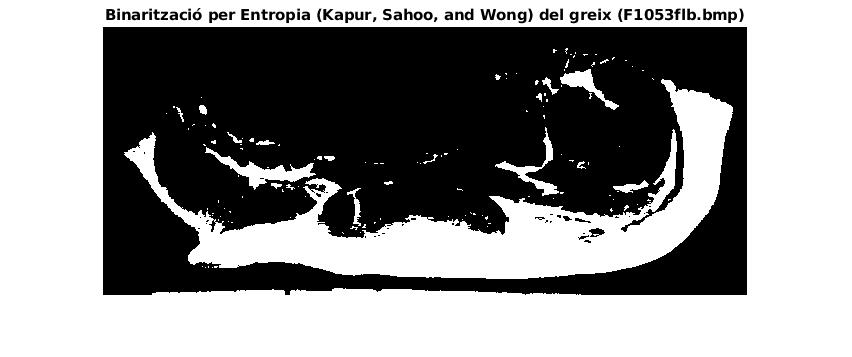
\includegraphics[scale=0.45]{output/KapurF1053flb.jpg}
    \vspace*{-1.3cm}
  \caption{Kapur}
  \label{fig:Kapur}
\end{figure}
\begin{figure}[H]
\centering
  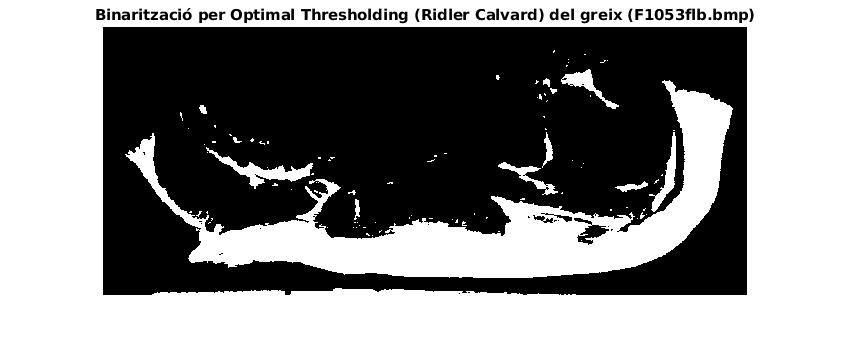
\includegraphics[scale=0.45]{output/OptimalF1053flb.jpg}
  \vspace*{-1.3cm}  
  \caption{Optimal}
  \label{fig:Optimal}
\end{figure}
\begin{figure}[H]
\centering  
  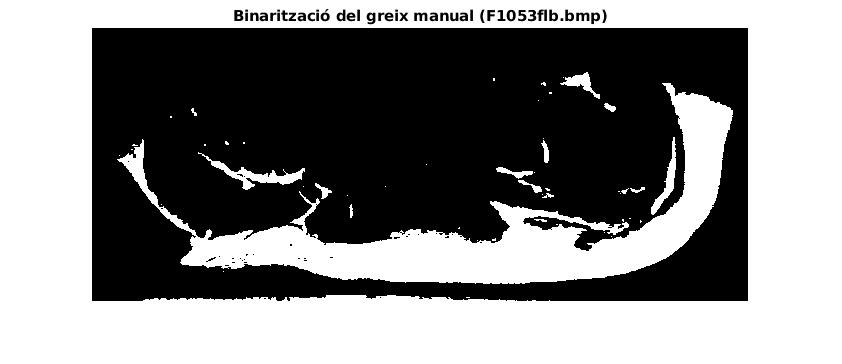
\includegraphics[scale=0.45]{output/ManualF1053flb.jpg}
   \vspace*{-1.3cm}
  \caption{Manual}
  \label{fig:Manual}

\end{figure}
\begin{figure}[H]
\centering
  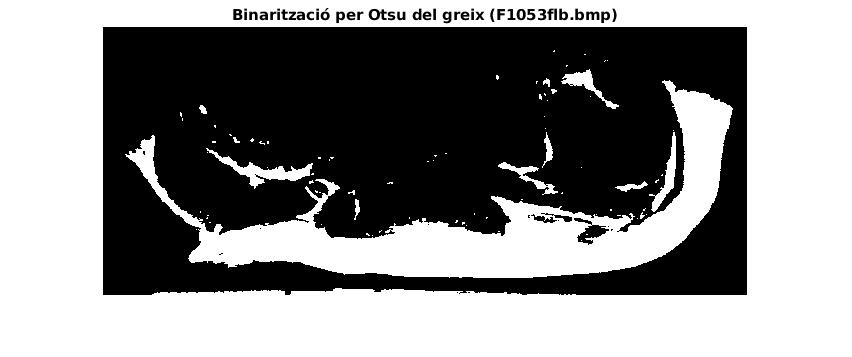
\includegraphics[scale=0.45]{output/OtsuF1053flb.jpg}
  \vspace*{-1.3cm} 
  \caption{Otsu}
  \label{fig:Otsu}
\end{figure}

\begin{figure}[H]
\centering
  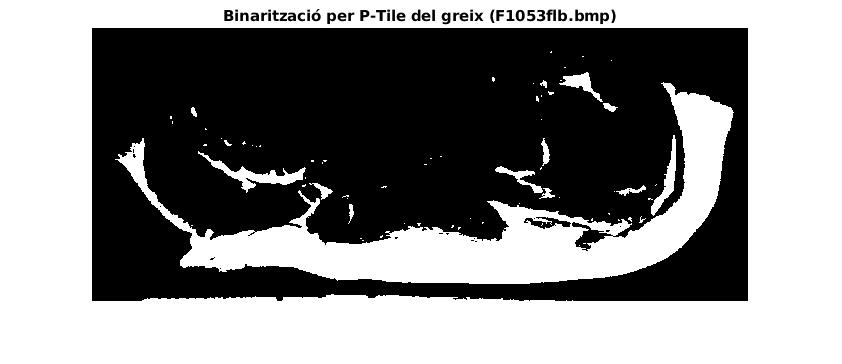
\includegraphics[scale=0.45]{output/PtileF1053flb.jpg}
  \caption{Ptile}
  \label{fig:Ptile}
    \vspace{-0.3cm}
\end{figure}
\newpage
\begin{thebibliography}{100}

\bibitem{A Comparison of Thresholding Methods - NTNU}
C. Henden (2004). \textit{ Exercise in Computer Vision. A Comparison of Thresholding Methods.} [online] NTNU. Available at: http://www.pvv.org/~perchrh/papers/datasyn/paper2/report.pdf [Accessed 14 Mar. 2019].


\bibitem{Analysis of image Thresholding Methods for application to augmented reality enviornments}
D. Martín Carabias (2012). \textit{Analysis of image Thresholding Methods for application to augmented reality enviornments.} [online] UCM. Available at: https://eprints.ucm.es/16932/1/Tesis\_Master\_Daniel\_Martin\_Carabias.pdf [Accessed 14 Mar. 2019].


\bibitem{A survey of Thresholding Techniques}
P. K. Sahoo, S. Soltani, K.C. Wong and Y.C. Chen (1988). \textit{A survey of Thresholding Techniques}. University of Waterloo, Waterloo, Canada  [Accessed 16 Mar. 2019].

\bibitem{}N. Otsu, \textit{A Threshold Selection Method from Gray-Level Histograms}, in IEEE Transactions on Systems, Man, and Cybernetics, vol. 9, no. 1, pp. 62-66, Jan. 1979.
[online] Available at http://ieeexplore.ieee.org/stamp/stamp.jsp?tp=\&arnumber=4310076\&is
number=4310064 [Acessed 17 Mar. 2019].

\bibitem{}Dr. Andrew Greensted (2010), \textit{Otsu Thresholding}. [online]. Available at http://www.labbookpages.co.uk/software/imgProc/otsuThreshold.html [Accessed 17 Mar. 2019].

\bibitem{}Senthilkumaran,  N.  \&  Sivapriya,  M.  (2017),  \textit{Riddler's  Thresholding Algorithm  for  DNA  Image  Using  ISODATA  Modified  Algorithm} Journal  of Information Technology, Vol.3, No.2, pp.41-48. [online] Available at: http://www.ijitjournal.org/volume-3/issue-2/IJIT-V3I2P9.pdf [Accessed 17 Mar. 2019].

\end{thebibliography}

\end{document}